\documentclass[UTF8,a4paper,11pt,fontset=windows]{ctexart}
\usepackage[a4paper,top=19mm,bottom=18mm,left=18mm,right=18mm,headheight=22pt]{geometry}
\usepackage{amsmath,amssymb,graphicx,booktabs,tabularx,longtable}
\usepackage[table]{xcolor}
\usepackage{enumitem,titlesec,fancyhdr,hyperref,url,tcolorbox,caption,float,microtype}
\definecolor{DeepInk}{HTML}{19313B}
\definecolor{Teal}{HTML}{0F6B67}
\definecolor{Coral}{HTML}{D4664A}
\definecolor{Green}{HTML}{3A8D5D}
\definecolor{SoftGray}{HTML}{F3F6F5}
\definecolor{PaleGold}{HTML}{FFF6DC}
\definecolor{MidGray}{HTML}{67757B}
\hypersetup{colorlinks=true,linkcolor=Teal,urlcolor=Coral,pdftitle={BM3R1驱动的sRNA Shutdown模块 Wiki叙事版报告}}
\setlength{\parindent}{2em}
\setlength{\parskip}{0.32em}
\setlist[itemize]{leftmargin=2em,itemsep=0.15em}
\setlist[enumerate]{leftmargin=2.2em,itemsep=0.2em}
\renewcommand{\arraystretch}{1.18}
\captionsetup{font=small,labelfont={bf,color=Teal},skip=5pt}
\titleformat{\section}{\Large\bfseries\color{DeepInk}}{\thesection.}{0.5em}{}
\titleformat{\subsection}{\large\bfseries\color{Teal}}{\thesubsection}{0.5em}{}
\pagestyle{fancy}
\fancyhf{}
\fancyhead[L]{\small\color{MidGray}BM3R1/sRNA Shutdown Wiki叙事版}
\fancyhead[R]{\small\color{MidGray}2026-09-09}
\fancyfoot[C]{\small\color{MidGray}\thepage}
\renewcommand{\headrulewidth}{0.4pt}
\newcolumntype{Y}{>{\raggedright\arraybackslash}X}
\newcommand{\citebox}[1]{\textcolor{Teal}{[#1]}}
\newtcolorbox{takeaway}{colback=SoftGray,colframe=Teal,boxrule=0.8pt,arc=1.5mm,left=3mm,right=3mm,top=2.5mm,bottom=2.5mm}
\newtcolorbox{pending}{colback=PaleGold,colframe=Coral,boxrule=0.8pt,arc=1.5mm,left=3mm,right=3mm,top=2.5mm,bottom=2.5mm}

\begin{document}
\begin{titlepage}
\thispagestyle{empty}
\vspace*{15mm}
{\color{Teal}\rule{28mm}{2.2pt}}\\[7mm]
{\fontsize{25}{31}\selectfont\bfseries\color{DeepInk}BM3R1驱动的sRNA Shutdown模块}\\[3mm]
{\fontsize{20}{26}\selectfont\bfseries\color{Teal}从持续状态到可调表达窗口}\\[8mm]
{\large\color{MidGray}面向iGEM Wiki叙事与模型评审的重组版本}\\[10mm]
\begin{tabular}{@{}ll@{}}
\textbf{版本} & Wiki叙事版 v1.1\\
\textbf{日期} & 2026-09-09\\
\textbf{用途} & Model页面正文底稿与技术附件\\
\textbf{研究性质} & 文献锚定的确定性ODE与条件性参数分析
\end{tabular}
\vspace{12mm}
\begin{tcolorbox}[colback=DeepInk,colframe=DeepInk,arc=1.5mm,boxrule=0pt,left=5mm,right=5mm,top=4mm,bottom=4mm]
{\color{white}\bfseries 一句话结论}\\[2mm]
{\color{white}BM3R1下降能够解除对RyhB的抑制，使RyhB消耗目标mRNA，并把持续LR输出转化为有限、可调的新生翻译窗口。基准FWHM为6.98 h，LR后期新生翻译残留为17.0\%，但这些是机制级预测，不是wet-lab验证。}
\end{tcolorbox}
\vfill
{\small\color{MidGray}本版突出“问题--机制--校验--设计决策--边界”的Wiki证据链；完整扫描和参数审计保留在技术报告与CSV中。}
\end{titlepage}

\section*{核心故事}
\begin{takeaway}
\textbf{问题：}DNA计数状态是稳定的，直接连接输出会让目标mRNA在整个LR阶段持续产生。\\
\textbf{设计：}利用PB转LR后BM3R1自然下降，解除Shutdown promoter抑制并产生RyhB。\\
\textbf{结果：}当前单bit测试中，新生翻译窗口由10.61 h缩短为6.98 h，峰值保留98.6\%，5/5受审周期仍一次输入一次完整反转。\\
\textbf{设计规则：}有效RyhB供给$\alpha_SC/\alpha_M$必须高于目标mRNA供给；4--8是当前参数包络中优先验证的区间。
\end{takeaway}

\begin{pending}
\textbf{尚待实验组决定：}当前模型是单个PB/LR bit的局部Shutdown读出。Shutdown最终连接哪一位、哪一个计数状态或哪一种状态解码器尚未确定，因此本报告不声称已经完成“计数到指定数字$N$后只输出一次”的完整逻辑。
\end{pending}

\begin{takeaway}
\textbf{10.61 h不是完整系统的表达上限：}当前单bit每次输入就在PB与LR间交替，因此无Shutdown对照只覆盖约一个LR驻留间隔。多bit状态若连续多个计数周期保持输出有效，无Shutdown表达可能远长于10.61 h；准确长度须在计数位、目标状态和复位逻辑确定后重算。Shutdown的核心价值是让新翻译无需等待DNA离开目标状态即可自行停止。
\end{takeaway}

\section{工程问题与机制}
如果输出基因直接由LR状态驱动，LR的DNA记忆会让输出持续存在。本方案不额外增加独立计时器，而是复用计数器为了延迟RDF而已有的BM3R1动态：PB状态下BM3R1高并抑制Shutdown promoter；PB转LR后BM3R1停止产生并下降，RyhB随后积累并与目标mRNA共同降解。

\begin{figure}[H]\centering
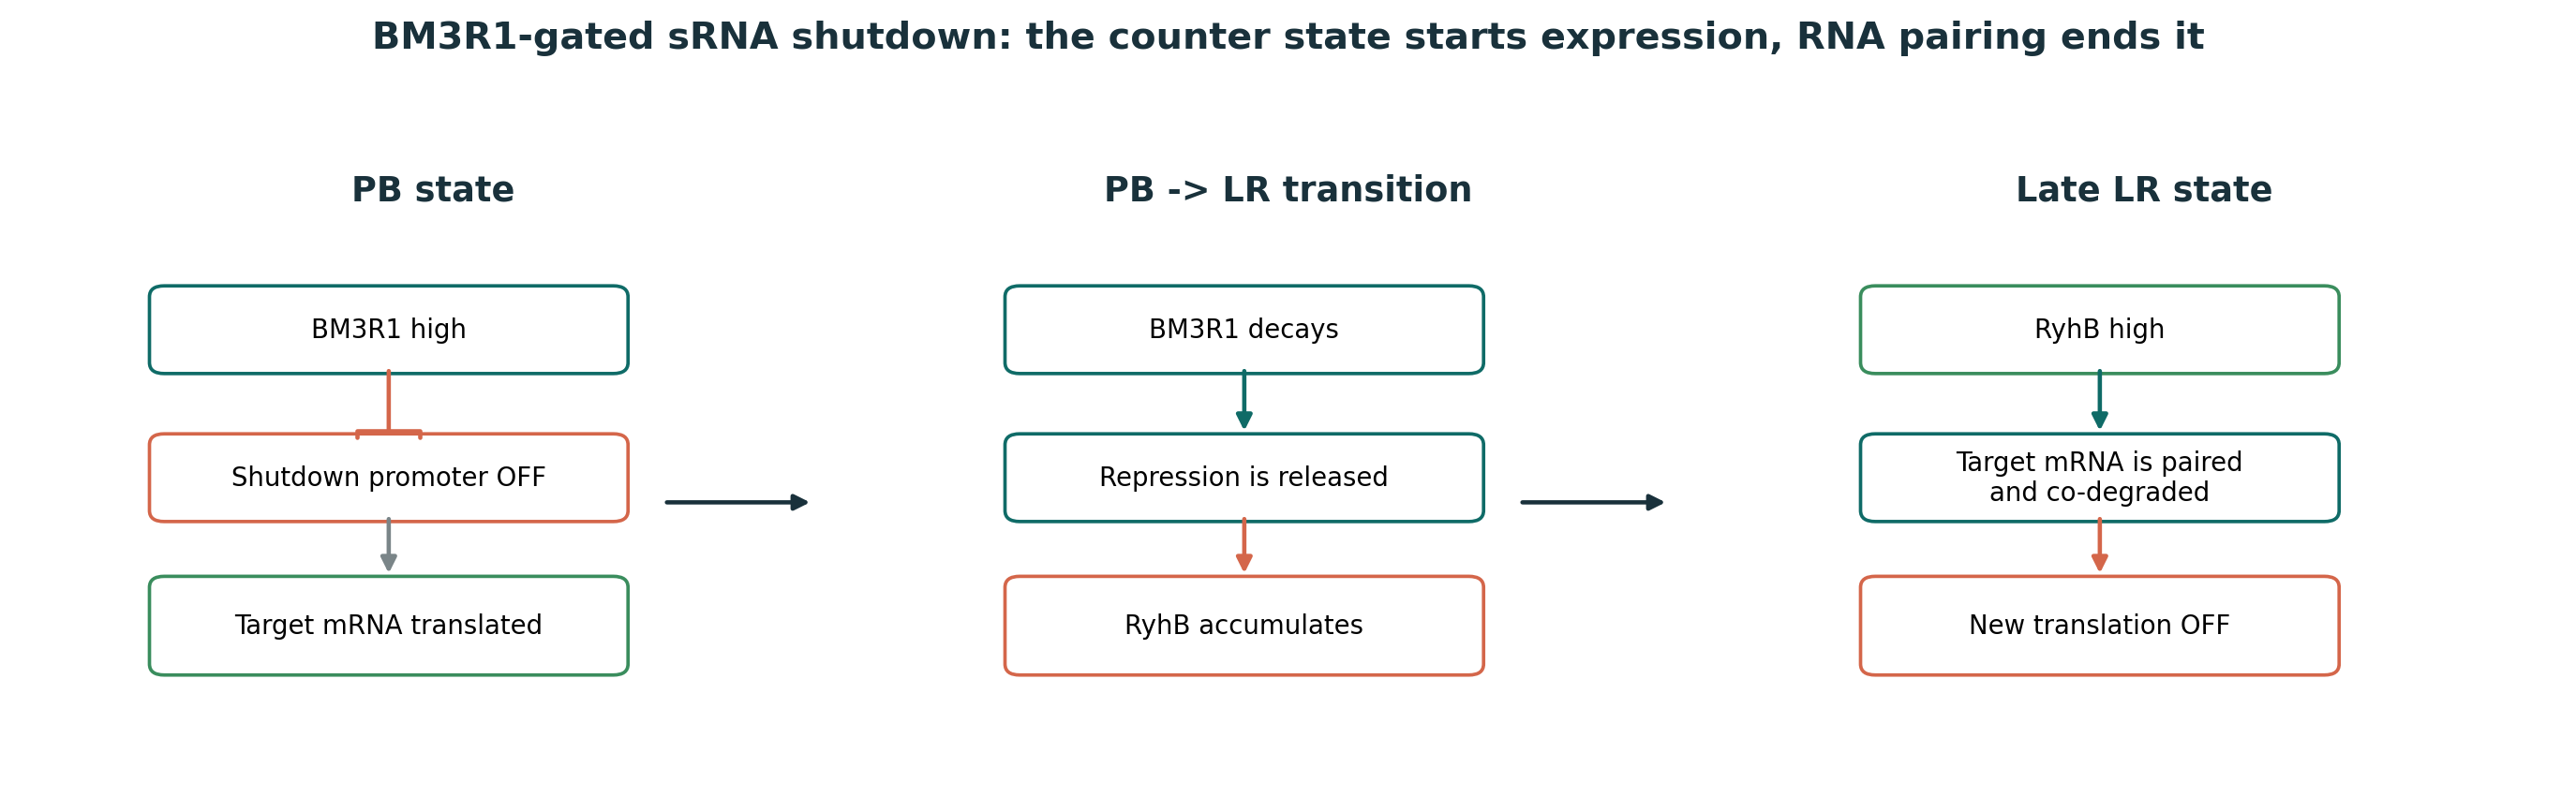
\includegraphics[width=0.98\textwidth]{assets/00_shutdown_mechanism.png}
\caption{BM3R1门控的sRNA Shutdown。计数状态启动输出，RNA共同降解结束新的翻译。}
\end{figure}

Shutdown关闭的是mRNA与新生翻译，不会主动清除已经合成的稳定蛋白。这一表述贯穿后续所有结果，避免把“翻译窗口”误写成“蛋白消失时间”。

\section{模型构建}
振荡器向38状态$\phi$C31/RDF计数器提供C31翻译通量：
\begin{equation}
v_{\mathrm{Int}}(t)=0.45v_{31}(t).
\end{equation}
计数器反应网络基于Zhao等人的单输入二进制计数模型；C31 RBS比例、Integrase标签损失率和BM3R1/RDF表达参数是本项目筛选的工程工作点，并非论文原始常数\citebox{Zhao 2019}。

BM3R1门控函数与新增的三个状态为：
\begin{align}
H(B)&=\ell+(1-\ell)\frac{1}{1+[B/(r_KK_{\mathrm{RDF}})]^n},\\
\frac{dS}{dt}&=\alpha_SH(B)-\beta_SS-pkSM,\\
\frac{dM}{dt}&=\alpha_Mf_{LR}-\beta_MM-kSM,\\
\frac{dO}{dt}&=\beta_{tr}M-(\delta_O+\mu)O.
\end{align}
其中$S$为RyhB，$M$为目标mRNA，$O$为归一化蛋白读出。配对通量$kSM$同时消耗mRNA和sRNA；$p=1$是Levine理论中的理想一对一极限，不是实验辨识常数。扩展分析另扫描$p=0.5$--1\citebox{Levine 2007}。

\section{文献基准与实现校验}
使用Levine给出的RyhB/sodB参数，在恒定满诱导下计算稳态。有限配对速率模型重现了文献描述的平滑阈值响应：当目标mRNA转录供给低于RyhB供给时，目标mRNA接近关闭；超过阈值后，剩余mRNA开始积累。

\begin{figure}[H]\centering
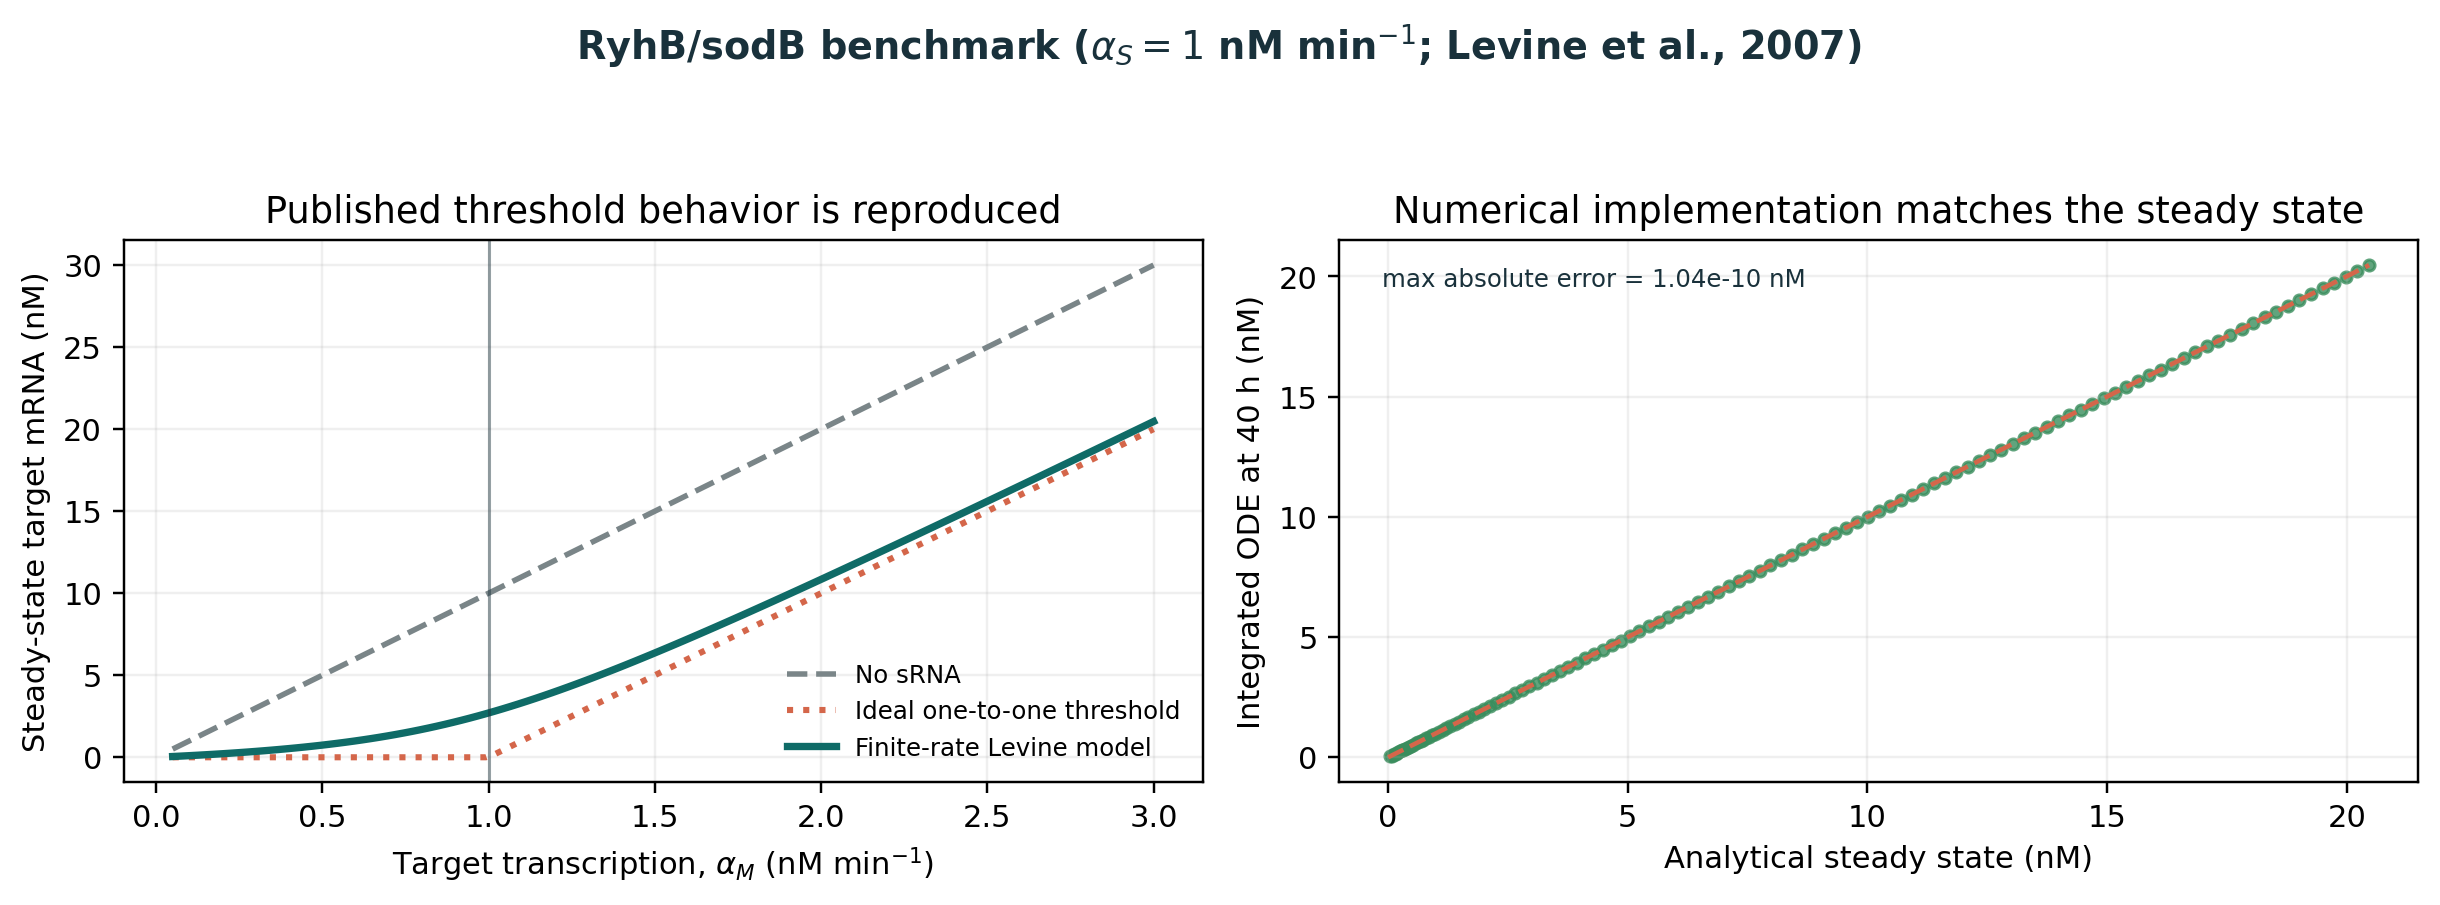
\includegraphics[width=0.96\textwidth]{assets/01_levine_threshold_validation.png}
\caption{Levine方程基准与数值实现。解析稳态和40 h ODE积分的最大mRNA绝对误差为$1.04\times10^{-10}$ nM。}
\end{figure}

\begin{takeaway}
该校验证明ODE实现与解析模型一致，并能重现Levine模型的阈值机制；它不是独立wet-lab验证，也不证明BM3R1 promoter能够实现全部扫描转录率。
\end{takeaway}

\section{参数与序列边界}
{\footnotesize
\begin{longtable}{@{}p{0.12\textwidth}p{0.14\textwidth}p{0.27\textwidth}p{0.39\textwidth}@{}}
\toprule
参数 & 模型基准 & 文献原值与换算 & 直接来源及底层依据\\\midrule
\endfirsthead
\toprule
参数 & 模型基准 & 文献原值与换算 & 直接来源及底层依据\\\midrule
\endhead
$\alpha_S$ & 0.06 $\mu$M h$^{-1}$ & $1\times60/1000=0.06$；文献范围0.1--10 nM min$^{-1}$ & Levine Figure 1C、Table 1与参数估计小节\citebox{Levine 2007}\\
$\alpha_M$ & 0.03 $\mu$M h$^{-1}$ & 项目取0.5 nM min$^{-1}$，$0.5\times60/1000=0.03$ & Levine由10--20 copies cell$^{-1}$估计约1 nM min$^{-1}$；底层转录组为Zhang 2005与Selinger 2000\citebox{Levine; Zhang; Selinger}\\
$\beta_S$ & 1.2 h$^{-1}$ & Levine取$1/50\approx0.02$ min$^{-1}$；$0.02\times60=1.2$ & Levine参数估计小节；约30 min RyhB半衰期依据Massé 2003与Moll 2003。沿用论文近似率，不重算$\ln2/t_{1/2}$\citebox{Levine; Massé; Moll}\\
$\beta_M$ & 6 h$^{-1}$ & Levine由约6 min半衰期取$1/10\approx0.1$ min$^{-1}$；$0.1\times60=6$ & Levine参数估计小节；底层sodB实验为Massé 2003\citebox{Levine; Massé}\\
$k$ & 1200 $\mu$M$^{-1}$h$^{-1}$ & $1/50=0.02$ nM$^{-1}$min$^{-1}$；$0.02\times1000\times60=1200$ & Levine根据Massé中RyhB约3 min内消失及靶mRNA约20 nM推得；非直接结合测量\citebox{Levine; Massé}\\
$p$ & 1；扫描0.5--1 & 理论一对一极限；无单位换算 & Levine理论模型情形，非实验辨识常数\citebox{Levine 2007}\\
$n$ & 3.1 & 直接采用 & Shin B3-BM3R1 gate拟合参数\citebox{Shin 2020}\\
leak & 0.00833 & $0.005/0.6=0.00833$ & 由Shin同一gate的$y_{min}/y_{max}$归一化\citebox{Shin 2020}\\
$r_K$ & 1；扫描0.5--2 & 无绝对单位换算 & 复用RDF operator的项目假设；非文献常数\\
cassette剂量$C$ & 1 & 无单位换算 & 每个counter plasmid一个cassette的项目假设\\
\bottomrule
\end{longtable}}

单位换算只改变数值表示，不提高证据等级。表中因此分别列出论文原始估计、论文引用的底层实验和本项目选择的设计点。

BM3R1的阈值在Shin文献中以RPU表示，不能无标定地转换为本模型的浓度单位。因此只使用Hill系数和归一化leak，并以相对阈值$r_K$进行扫描\citebox{Shin 2020}。

RyhB参考采用\textit{E. coli} K-12 MG1655当前NCBI注释：Gene ID 2847761，长度95 nt。Levine构建记载为RyhB $+1..+96$和\nolinkurl{sodB -1..+88}靶控制区。ODE不读取逐碱基序列，而是把序列、Hfq和RNase E作用折叠进有效$k$。因此95/96 nt边界不影响当前数值，但未来合成需回查原质粒；更换靶序列后也不能直接沿用当前$k$\citebox{NCBI; Hao 2011}。

\section{指标如何计算}
所有指标按稳定阶段的单次PB转LR事件计算：跳过第一个瞬态事件，以LR fraction向上穿越0.5定义开始；FWHM是单周期新生翻译通量高于自身半峰值的首末时间差；LR后期残留是LR仍有效时最后20\%区间的平均新生翻译通量除以峰值。

工程通过标准为：存在有限FWHM、LR后期残留低于20\%、峰值不低于对应无Shutdown对照的50\%。20\%和50\%是项目判据，不是文献常数。计数器则要求每个输入周期恰好一次状态穿越，并在周期末达到至少95\%目标状态。

\section{基准结果}
本节比较的是当前单bit轨迹，不是完整多bit计数器的最长表达时间。
\begin{table}[H]\centering
\begin{tabular}{@{}lrrr@{}}\toprule
指标 & 单bit无Shutdown & 单bit加Shutdown & 变化\\\midrule
新生翻译FWHM & 10.61 h & 6.98 h & 缩短34.2\%\\
LR后期新生翻译/峰值 & 97.9\% & 17.0\% & 降低82.6\%\\
新生翻译峰值 & 0.004999 & 0.004930 $\mu$M h$^{-1}$ & 保留98.6\%\\
稳定蛋白FWHM & 10.63 h & 7.33 h & 下降较慢\\
LR后期稳定蛋白/峰值 & 99.8\% & 32.0\% & 未低于20\%\\
\bottomrule\end{tabular}
\end{table}

34.2\%只表示同一单bit轨迹内的缩短幅度。若多bit译码让目标输出状态跨越$m$个输入间隔，无Shutdown持续时间可粗略写成$T_{\mathrm{no\ shutdown}}\sim mT_{\mathrm{input}}$，可能远长于10.61 h；具体$m$取决于尚未冻结的计数状态与复位逻辑。当前6.98 h是局部Shutdown动力学给出的关闭窗口，10.61 h则是本次单bit对照的状态驻留尺度。

5个受审周期都恰好发生一次完整反转；加入默认Shutdown operator负载后，计数器P score由0.995260变为0.995278。因此当前快速平衡负载模型没有显示Shutdown破坏计数行为。

\begin{figure}[H]\centering
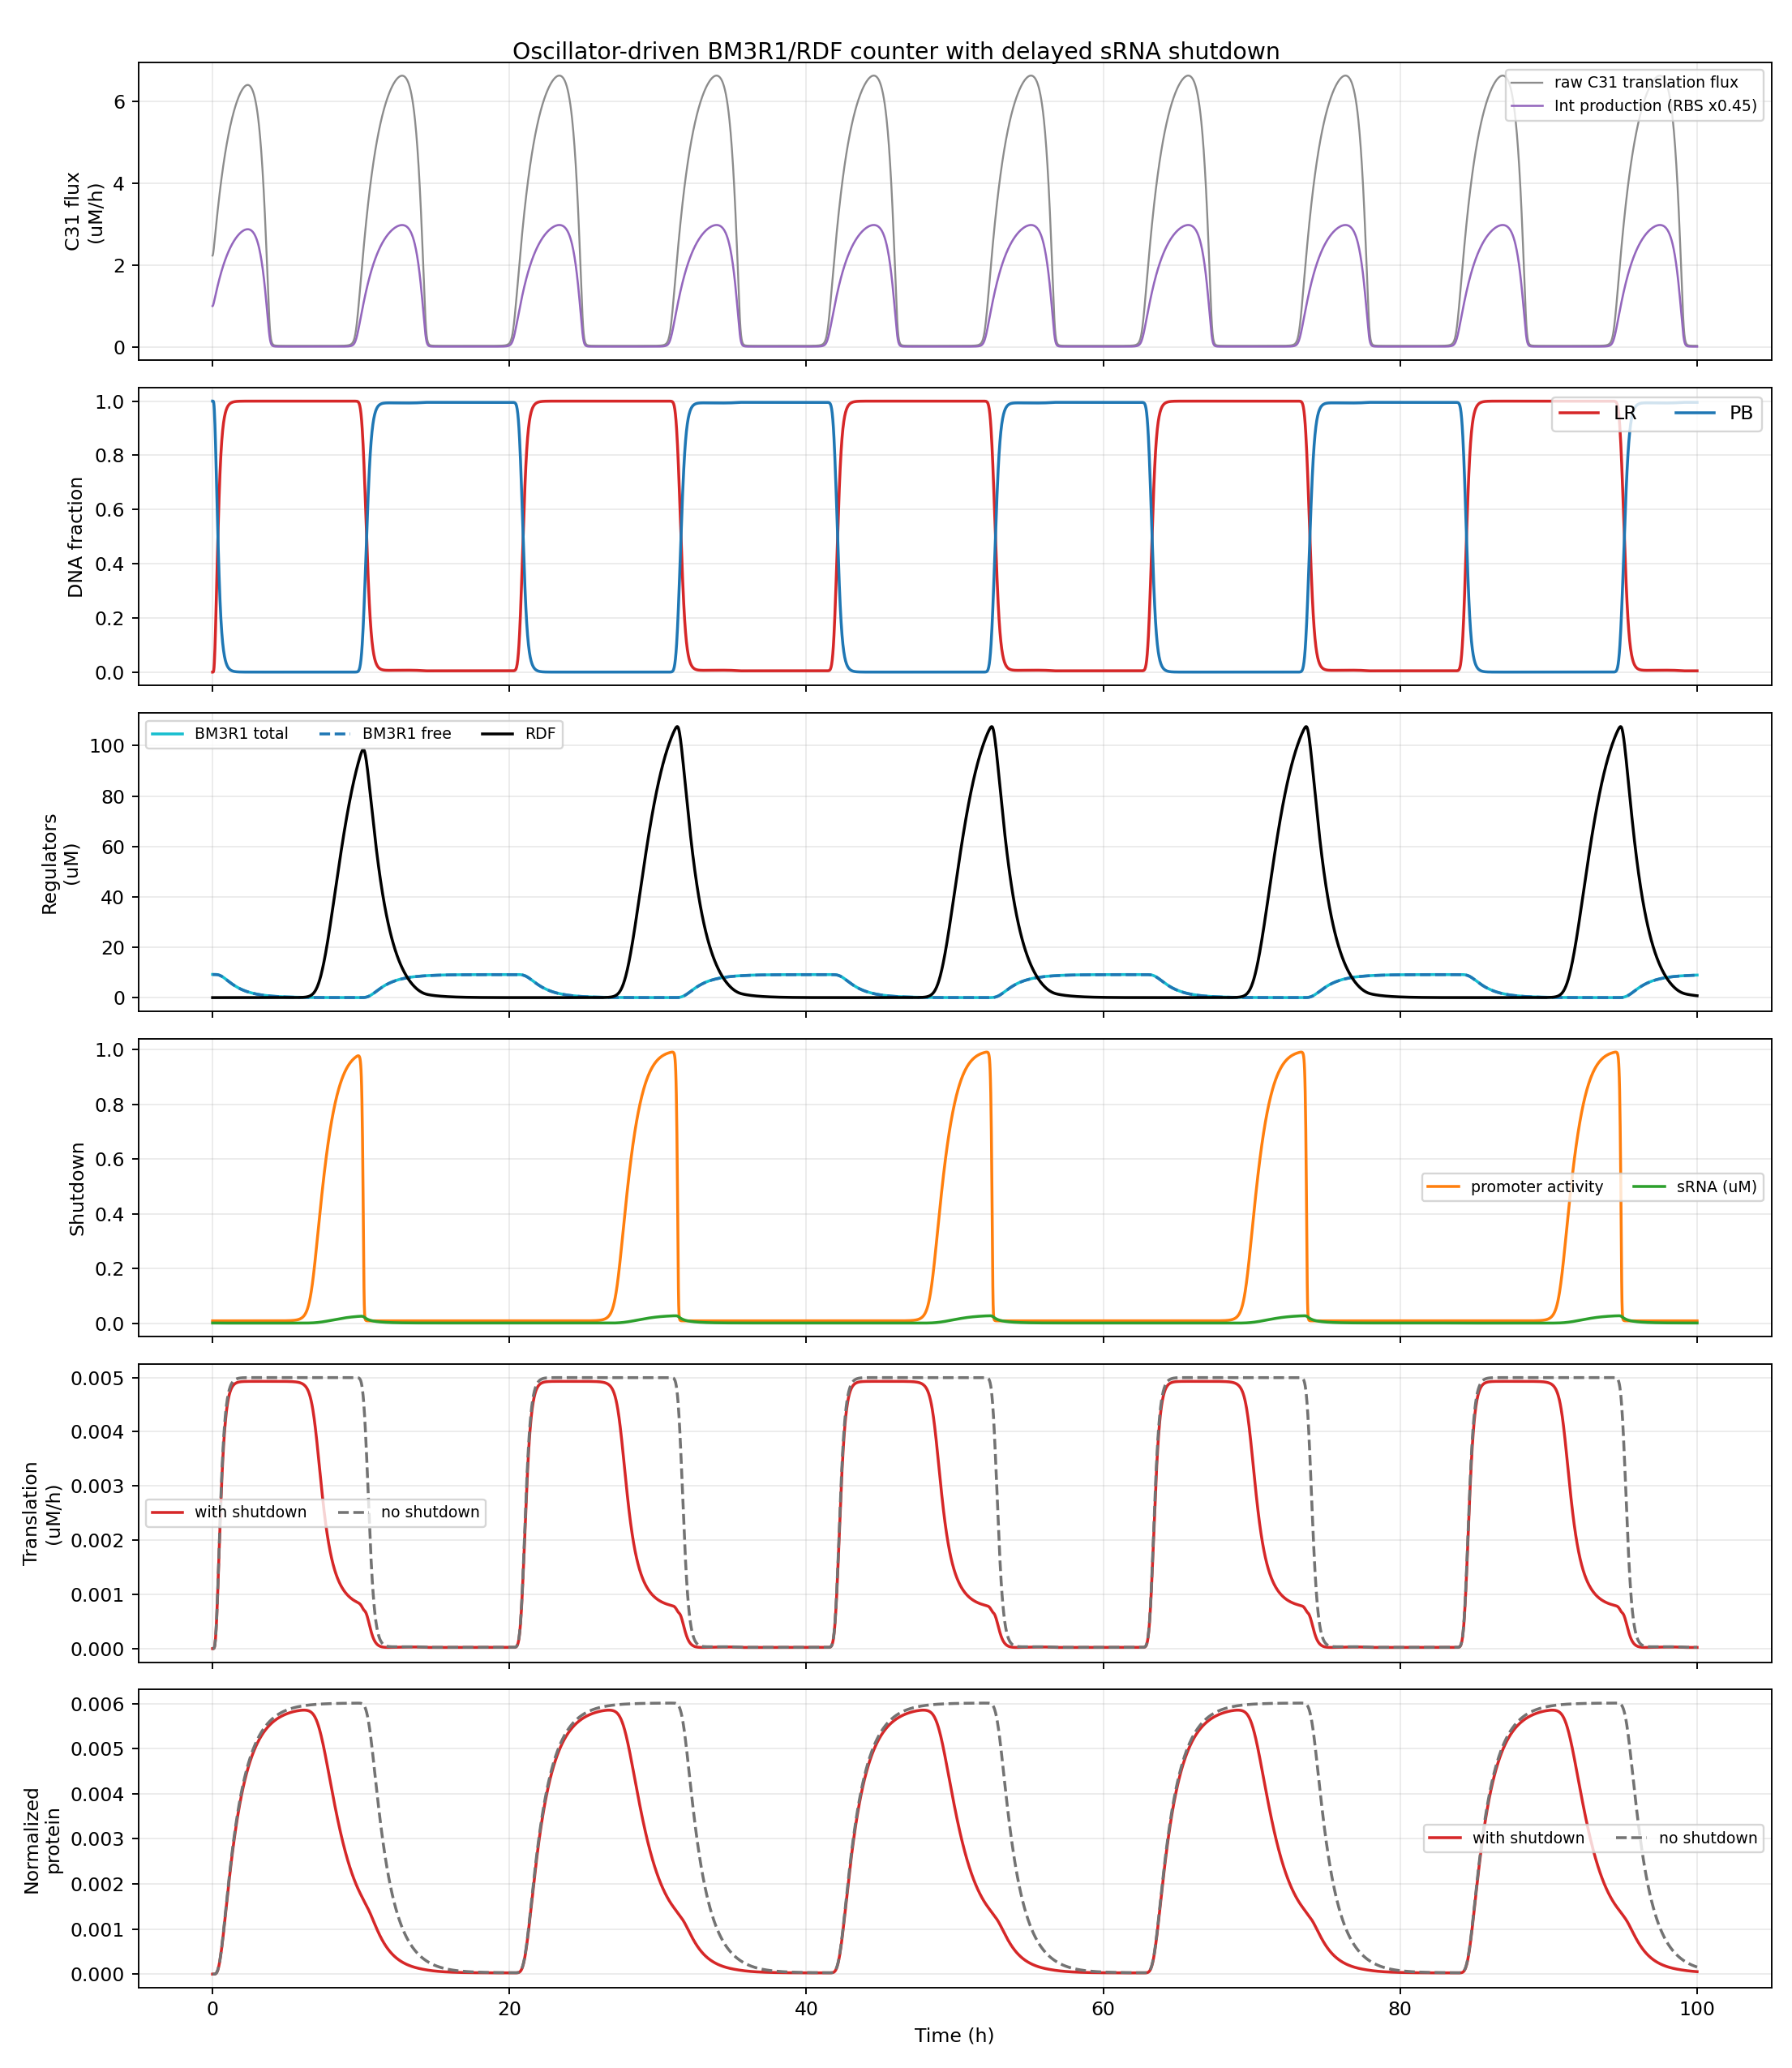
\includegraphics[width=0.94\textwidth]{assets/01_baseline_timecourse.png}
\caption{完整耦合时间过程。Shutdown保留前期输出并在LR后段停止新的翻译。}
\end{figure}

\section{可调性与设计窗口}
169个$\alpha_S-r_K$组合中有91个满足判据，新生翻译FWHM为5.42--7.36 h。提高RyhB转录率或提高相对BM3R1阈值，会更早解除Shutdown promoter抑制并缩短窗口。

\begin{figure}[H]\centering
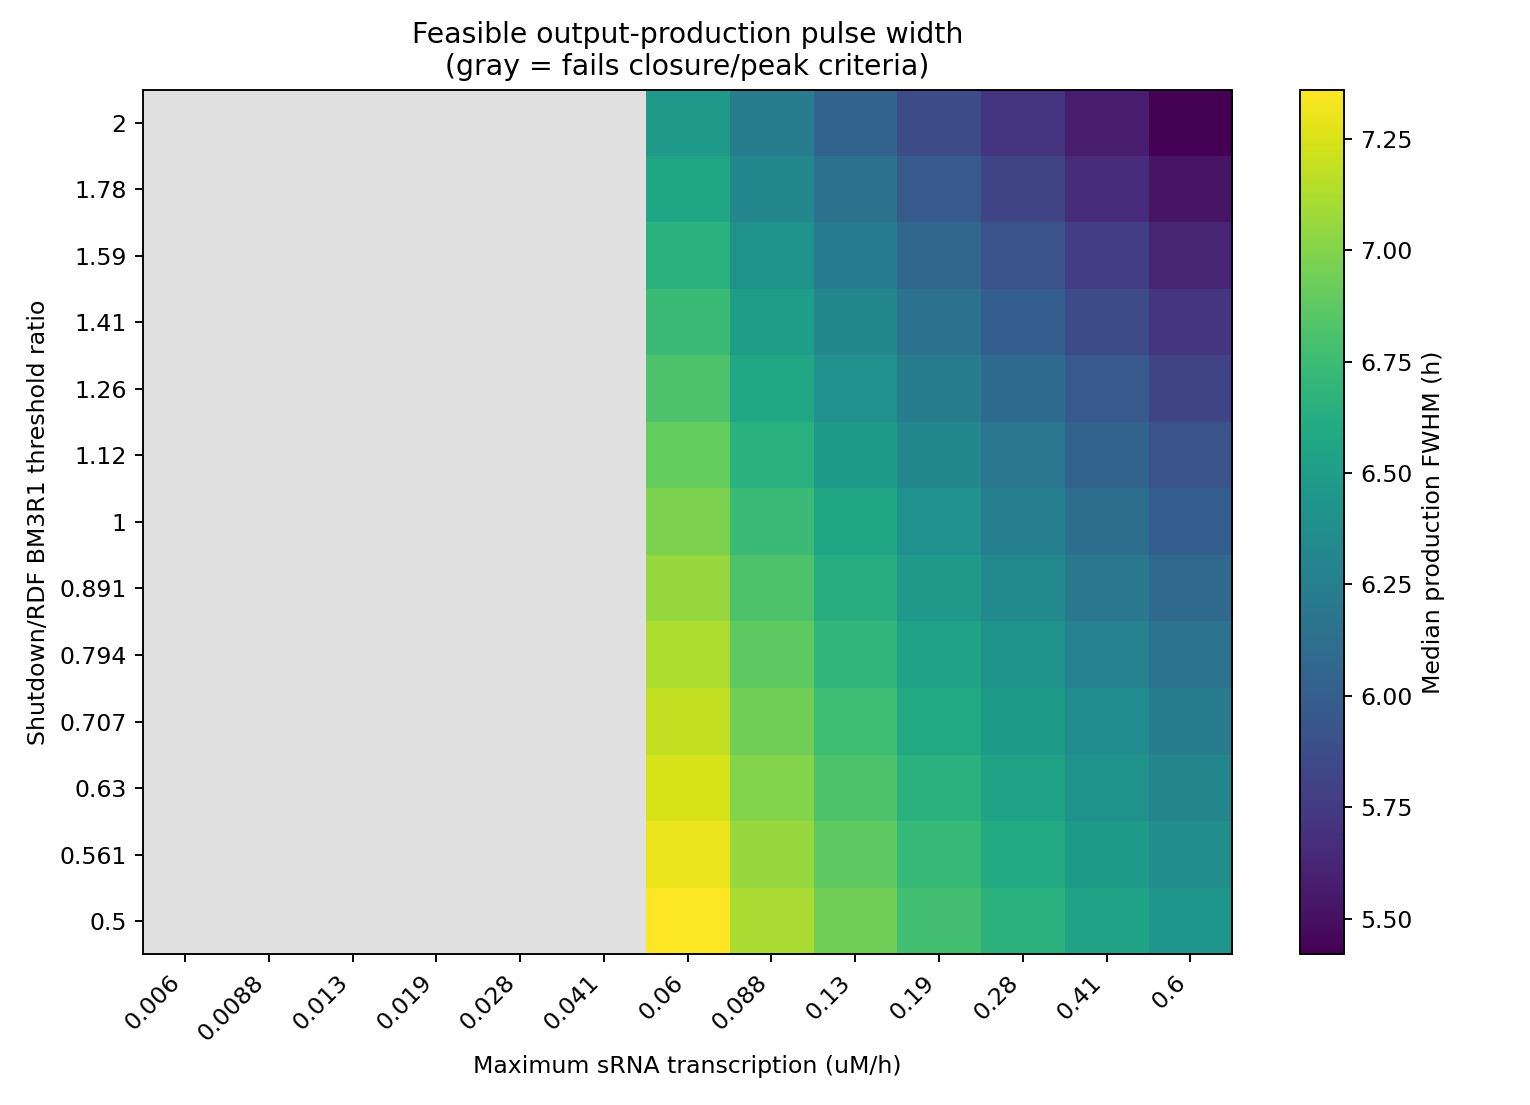
\includegraphics[width=0.73\textwidth]{assets/02_tunability_heatmap.png}
\caption{RyhB最大转录率和BM3R1相对阈值决定表达窗口。灰色区域未通过判据。}
\end{figure}

共同降解进一步给出有效供给比：
\begin{equation}
R_{\mathrm{supply}}=\frac{\alpha_SC}{\alpha_M}.
\end{equation}
225点供给扫描中有124点通过，离散网格最低可行比值为1.39，各靶转录水平最低可行比值的中位数为2.68。

\begin{figure}[H]\centering
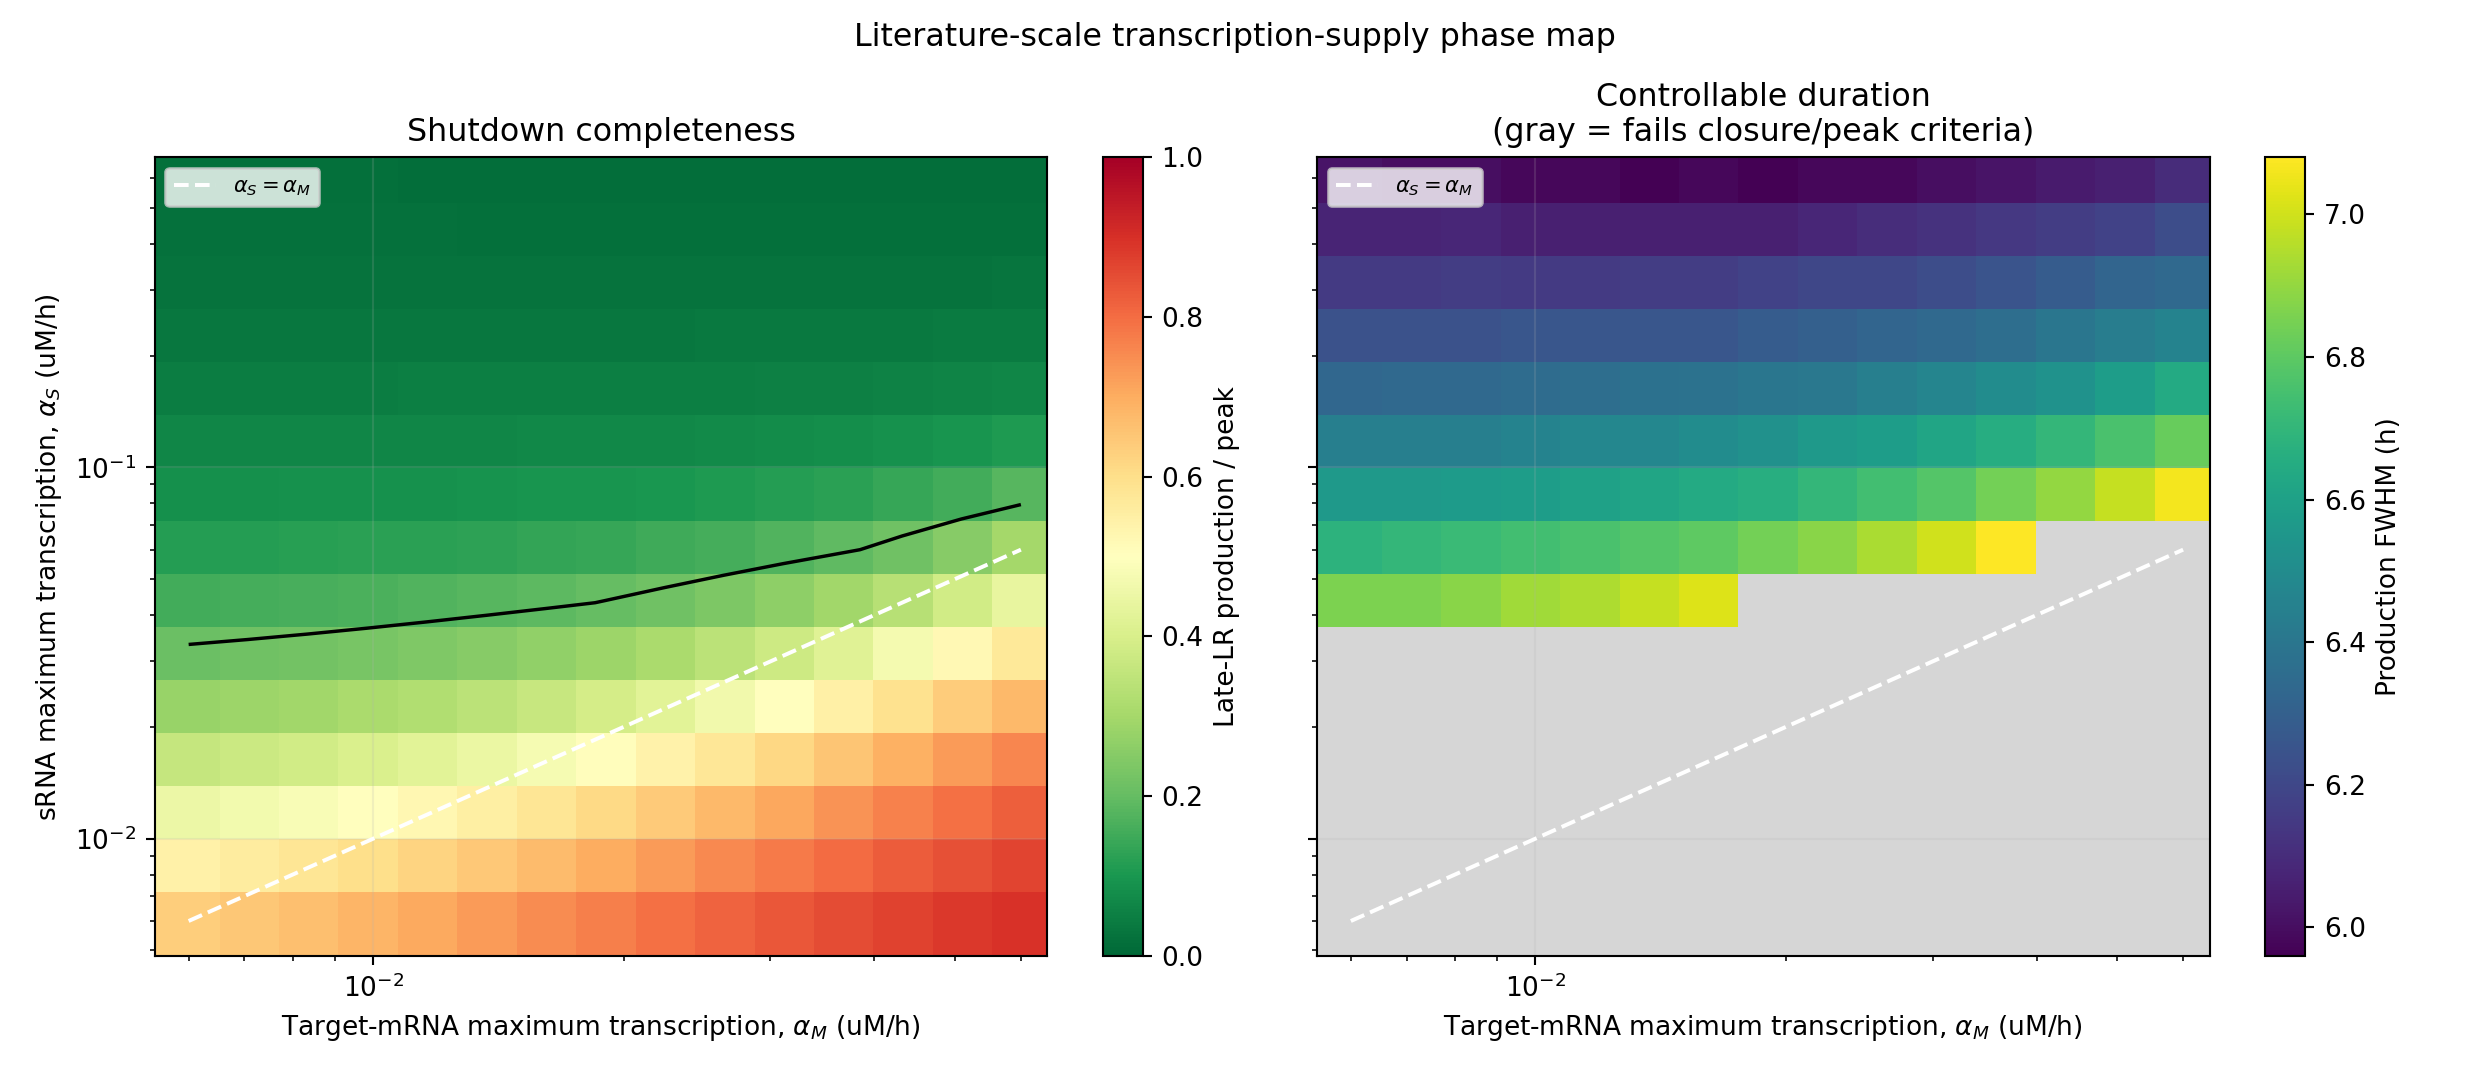
\includegraphics[width=0.96\textwidth]{assets/04_transcription_balance_phase_map.png}
\caption{转录供给相图。$\alpha_S=\alpha_M$附近通常不能可靠关闭。}
\end{figure}

\begin{table}[H]\centering\small
\begin{tabular}{@{}lrl@{}}\toprule
有效供给比 & 联合通过率 & 设计解释\\\midrule
$<1$ & 2.3\% & 应避免\\
1--2 & 23.0\% & 高度依赖其他参数\\
2--4 & 61.3\% & 有可行域，但需要筛选\\
4--8 & 91.7\% & 当前模型中优先验证的区间\\
$\geq8$ & 89.0\% & 关闭完整，但部分组合损失峰值\\
\bottomrule\end{tabular}
\end{table}
这些比例是所声明参数包络的覆盖率，不是实验成功概率。

\section{联合包络、生长与负载}
512点拉丁超立方抽样中，277点满足关闭和峰值标准；脉宽中位数为6.86 h，RyhB最大转录率是首要参数。参数被独立组合，故该分析不是实验后验分布。

\begin{figure}[H]\centering
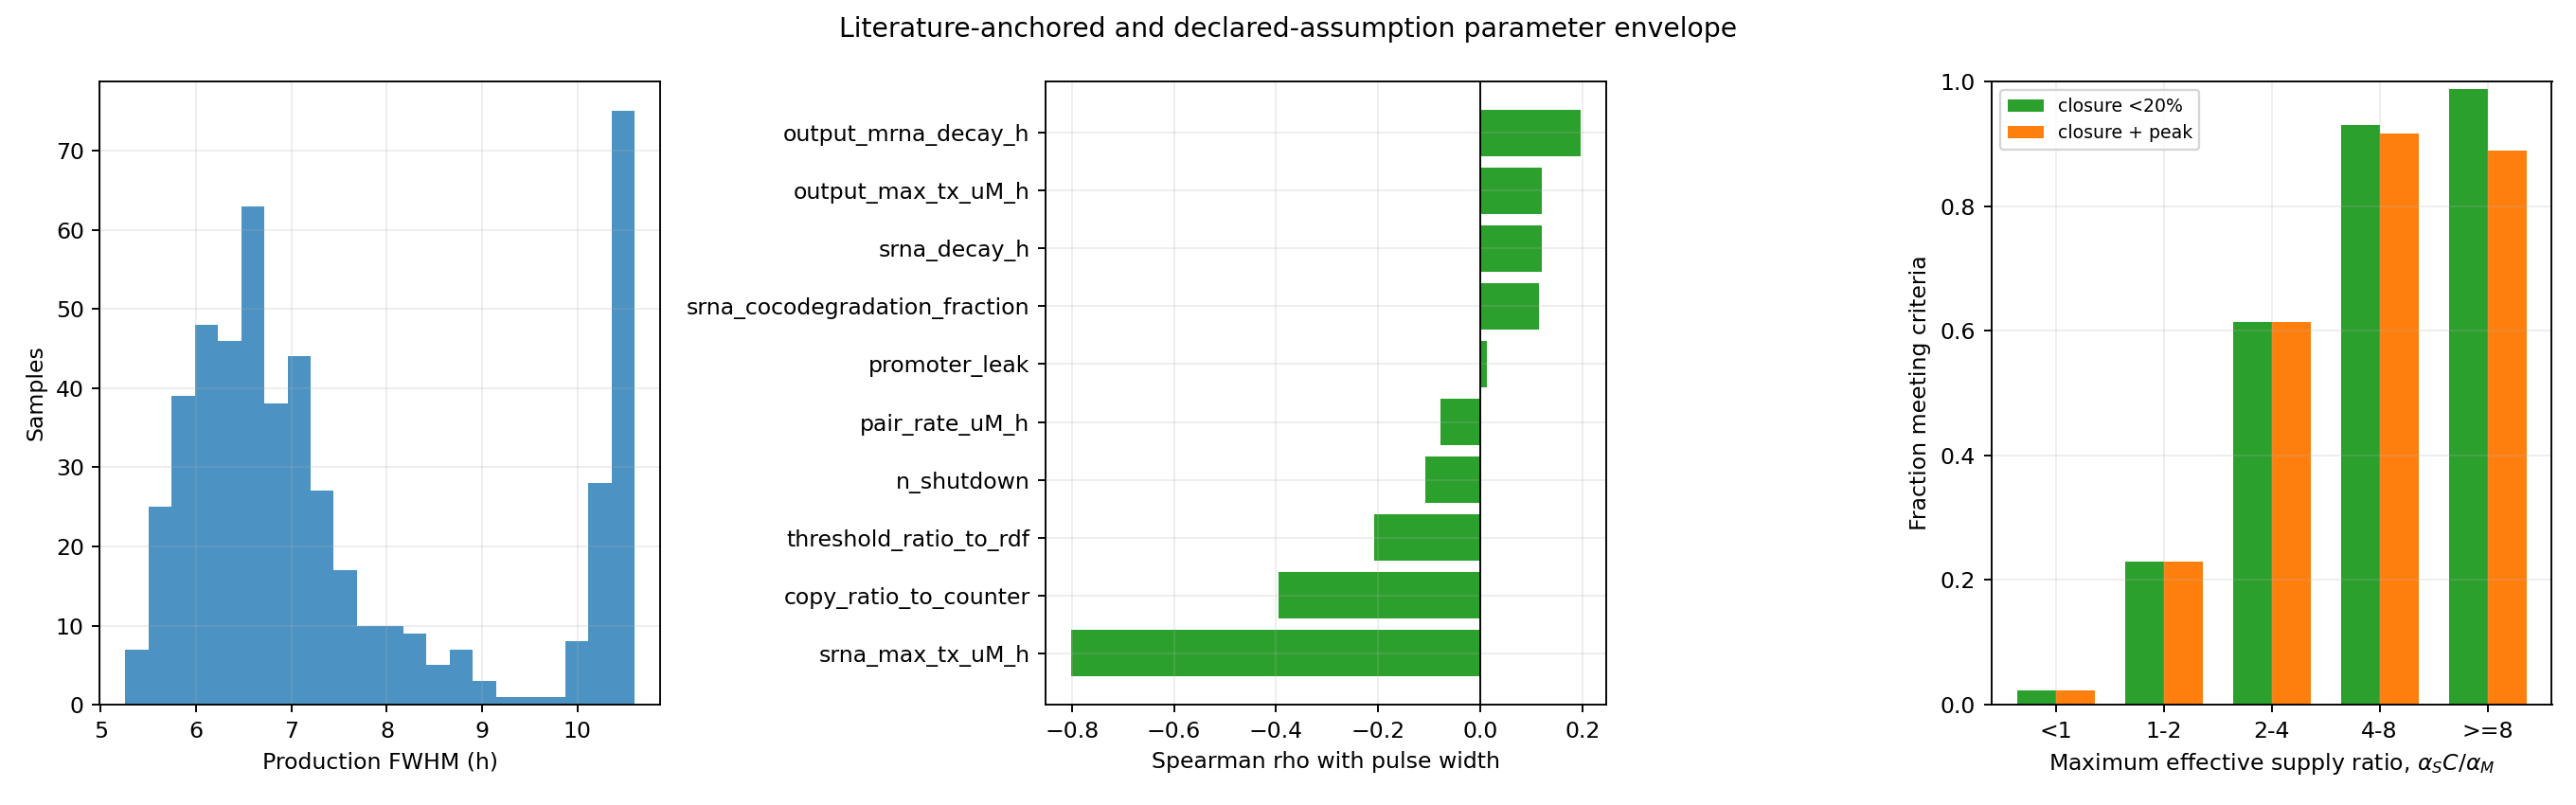
\includegraphics[width=0.88\textwidth]{assets/07_shutdown_joint_uncertainty.png}
\caption{512点参数包络。右图区分关闭完整度与关闭加峰值的联合标准。}
\end{figure}

在40、50和60 min倍增时间下，新生翻译FWHM分别为5.48、6.98和8.54 h，且均维持一峰一次反转。每种条件使用自己的无Shutdown对照。生长变慢会同步延长振荡周期和表达窗口，因此6.98 h不能被视为跨培养条件的固定常数。

\clearpage
\section{模型如何改变设计}
\begin{longtable}{@{}p{0.42\textwidth}p{0.52\textwidth}@{}}
\toprule
模型发现 & 设计影响\\\midrule
持续LR状态不会产生有限输出 & 必须增加转录后Shutdown，不能只依赖DNA状态\\
共同降解会消耗RyhB & 方程必须包含$-pkSM$，不能把RyhB当作不耗竭催化剂\\
等转录供给通常不足 & 设计时显式计算$\alpha_SC/\alpha_M$\\
4--8供给比最稳定 & 优先在该区间选择或模拟promoter与cassette剂量\\
增加cassette剂量会占用BM3R1 & 先调RyhB promoter或operator阈值，高拷贝作为次选\\
生长速度影响绝对窗口 & 按预期培养条件重新标定\\
稳定蛋白不会被RyhB直接清除 & 如需快速下降，应指定蛋白并加入有依据的降解标签\\
\bottomrule
\end{longtable}

最核心的工程贡献不是给出一个固定脉宽，而是确定：\textbf{RyhB有效转录供给必须超过目标mRNA供给，并在关闭完整度与峰值保留之间权衡。}

\section{结论边界与下一步}
当前结果支持“在文献量级和声明假设下，BM3R1驱动的RyhB Shutdown存在明确机制可行域”。它不支持以下表述：构建已被实验验证、给定序列已被模型验证、54.1\%是实验成功率，或完整多位计数到目标次数的输出逻辑已经完成。

\begin{itemize}
\item 与实验组确定Shutdown连接的计数位或状态解码逻辑；
\item 若继续推进序列层设计，明确是否采用\nolinkurl{sodB -1..+88}目标接口并检查融合结构；
\item 在无wet-lab条件下，把BM3R1 RPU到RyhB转录率、Hfq容量和内源靶标竞争作为下一层情景模型；
\item 指定输出蛋白后，再决定是否需要蛋白降解标签。
\end{itemize}

\section{复现与Wiki部署}
核心脚本与机器可读输出包括：
\begin{itemize}
\item \nolinkurl{shutdown_core.py}、\nolinkurl{run_analysis.py}和\nolinkurl{run_extended_analysis.py}；
\item \nolinkurl{build_wiki_assets.py}；
\item \nolinkurl{00_parameter_provenance.csv}；
\item \nolinkurl{summary.json}和\nolinkurl{extended_summary.json}。
\end{itemize}

Wiki正文建议以机制图、Levine基准图、基准时间过程、供给相图、联合包络和设计决策表为主线；接口扫描、完整参数表和逐周期CSV放入折叠区或下载附件。这样页面首先回答“为什么做、模型改变了什么”，随后再提供方程和复现细节。

\section*{参考文献}
\begin{enumerate}[label={\arabic*.}]
\item Zhao, J. et al. \textit{Nucleic Acids Research} 47, 4896--4909 (2019). \url{https://doi.org/10.1093/nar/gkz245}
\item Levine, E. et al. \textit{PLoS Biology} 5, e229 (2007). \url{https://doi.org/10.1371/journal.pbio.0050229}
\item Shin, J. et al. \textit{Molecular Systems Biology} 16, e9401 (2020). \url{https://doi.org/10.15252/msb.20199401}
\item Hao, Y. et al. \textit{PNAS} 108, 12473--12478 (2011). \url{https://doi.org/10.1073/pnas.1100432108}
\item Mass\'e, E. et al. \textit{Genes \& Development} 17, 2374--2383 (2003). \url{https://doi.org/10.1101/gad.1127103}
\item Pr\'evost, K. et al. \textit{Genes \& Development} 25, 385--396 (2011). \url{https://doi.org/10.1101/gad.2001711}
\item NCBI Gene 2847761, \textit{ryhB}. \url{https://www.ncbi.nlm.nih.gov/gene/2847761}
\item Zhang, Z. et al. \textit{Journal of Bacteriology} 187, 980--990 (2005). \url{https://doi.org/10.1128/JB.187.3.980-990.2005}
\item Selinger, D. W. et al. \textit{Nature Biotechnology} 18, 1262--1268 (2000). \url{https://doi.org/10.1038/82367}
\item Moll, I. et al. \textit{RNA} 9, 1308--1314 (2003). \url{https://doi.org/10.1261/rna.5850703}
\end{enumerate}
\end{document}
